\section{Circle sizes}
\label{hdm_circle_size}
The main parameter for the Hausdorff distance mask method is the size of the circle that is applied onto the image. In this section we compare the sizes of 10, 15 and 20 pixels in diameter.

\begin{figure}[H]
    \centering
    \begin{subfigure}{.33\textwidth}
        \centering
        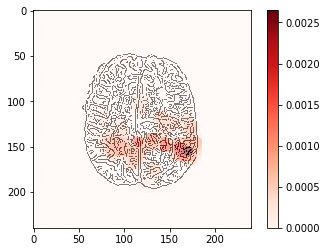
\includegraphics[width=\linewidth]{chapters/06_hdm/b_Brats18_TCIA08_242_1_L2/23.png}
        \caption{Pixel size }
    \end{subfigure}%
    \begin{subfigure}{.33\textwidth}
        \centering
        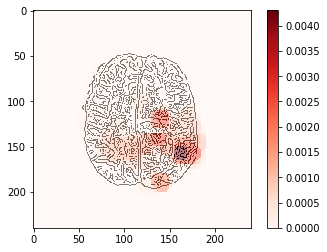
\includegraphics[width=\linewidth]{chapters/06_hdm/circle15/3.png}
        \caption{TODO}
    \end{subfigure}
        \begin{subfigure}{.33\textwidth}
        \centering
        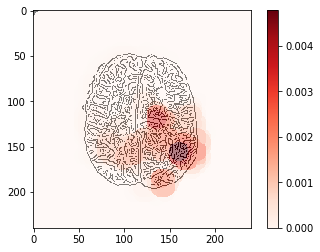
\includegraphics[width=\linewidth]{chapters/06_hdm/circle20/3.png}
        \caption{TODO}
    \end{subfigure}
    \caption{TODO}
\end{figure}

\begin{figure}[H]
    \centering
    \begin{subfigure}{.33\textwidth}
        \centering
        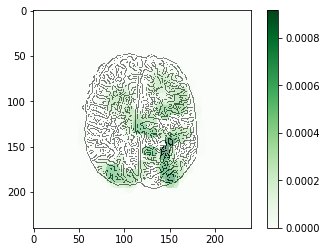
\includegraphics[width=\linewidth]{chapters/06_hdm/b_Brats18_TCIA08_242_1_L2/24.png}
        \caption{TODO}
    \end{subfigure}%
    \begin{subfigure}{.33\textwidth}
        \centering
        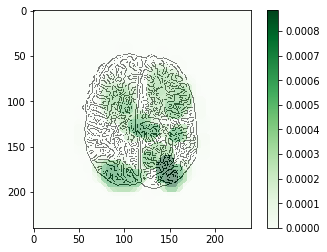
\includegraphics[width=\linewidth]{chapters/06_hdm/circle15/4.png}
        \caption{TODO}
    \end{subfigure}
        \begin{subfigure}{.33\textwidth}
        \centering
        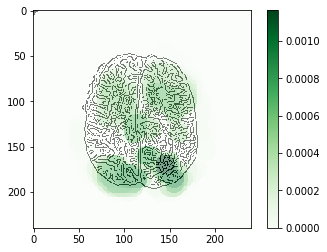
\includegraphics[width=\linewidth]{chapters/06_hdm/circle20/4.png}
        \caption{TODO}
    \end{subfigure}
    \caption{TODO}
\end{figure}
